\documentclass{article}
\usepackage{graphicx}
\usepackage[utf8]{inputenc}
\usepackage{amsmath, amssymb, latexsym}

\usepackage{pgfplots}
\usepackage{algorithm}
\usepackage[noend]{algpseudocode}
\usepackage{tikz}
\usepackage{nicefrac}
\pgfplotsset{every axis legend/.append style={
at={(0,0)},
anchor=north east}}
\usetikzlibrary{shapes,positioning,intersections,quotes}
\usetikzlibrary{arrows.meta,
                bending,
                intersections,
                quotes,
                shapes.geometric}
                
\definecolor{darkgreen}{rgb}{0.0, 0.6, 0.0}
\definecolor{darkred}{rgb}{0.7, 0.0, 0.0}
\makeatletter
\def\BState{\State\hskip-\ALG@thistlm}
\makeatother
\title{Week 4}
\begin{document}
  \pagenumbering{gobble}
  \maketitle
  \newpage
  \pagenumbering{arabic}

\section*{Linear regression with multiple features}
\begin{itemize}
\item Multiple variables = multiple features.
\item $x_1$ - size, $x_2$ - number of bedrooms, $x_3$ - number of floors, $x_4$ - age of home.
\item $n$ - number of features (n = 4).
\item $m$ - number of examples (i.e. number of rows in a table).
\item $x^i$ - vector of the input (in our example a vector of the four parameters for the $i^{th}$ input example), where $i$ is the training set's index.
\item $x_j^i$ the value of $j^{th}$ feature in the $i^{th}$ training set. For example $x_2^3$ represents the number of bedrooms in the third house.
\end{itemize}

~\\
Previously, our hypothesis had the following form:
$$h_{\theta}(x) = \theta_0 + \theta_1x$$

Now we have multiple features:
$$h_{\theta}(x) = \theta_0 + \theta_1x_1 + \theta_2x_2 + \theta_3x_3 + + \theta_4x_4$$

~\\
For convenience of notation, we can introduce $x_0 = 1$. As a result, your feature vector is now n + 1 dimensional and indexed from 0.

$$h_{\theta}(x) = \theta^T X$$

\section*{Gradient descent for multiple variables}

$$\quad J(\theta_0, \theta_1, ..., \theta_n) = \frac{1}{2m} \sum_{m}^{i=1}(h_{\theta}(x^{(i)}) - y^{(i)})^2$$

\begin{algorithm}
\caption{Gradient Descent}\label{euclid}
\begin{algorithmic}[1]
\Large
\While {not converged}
\State $\theta_j := \theta_j - \alpha \frac{\partial}{\partial \theta_j} J(\theta_0, ..., \theta_n)$.
\State $(for\ j = 0, ..., n)$
\EndWhile
\end{algorithmic}
\end{algorithm}

\begin{itemize}
\item For each $\theta_j$ (0 until n) we make an simultaneous update.
\item $\theta_j$ is now equal to it's previous value subtracted by learning rate ($\alpha$) times the partial derivative of of the $\theta$ vector with respect to $\theta_j$. 
\end{itemize}

\section*{Gradient Decent in practice: Feature Scaling}

\begin{itemize}
\item If you have a problem with multiple features, make sure they all have a comparable scale.
\item For example, x1 = size (0 - 2000 feet) and x2 = number of bedrooms (1-5). Means the contours generated if we plot $\theta_1$ vs. $\theta_2$ give a very tall and thin shape due to the huge range difference.
\item Finding the global minimum using gradient descent on this type of cost function might take a long time.
\end{itemize}

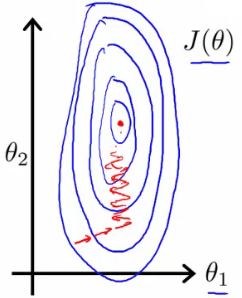
\includegraphics[width=0.3\textwidth]{resources/feature_scaling}

\subsection*{Mean normalization}

\begin{itemize}
\item Take a feature $x_i$.
\item Replace it by  \begin{Large} $\frac{x_i - mean}{max}$ \end{Large}.
\item So your values all have an average of about 0.
\end{itemize}

~\\
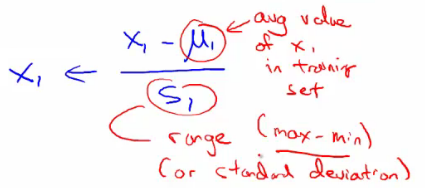
\includegraphics[width=\textwidth]{resources/mean_normalization}

\subsection*{Learning Rate $\alpha$}
\begin{itemize}

\item Plot the $min J(\theta)$ vs. the number of iterations (i.e. plot $J(\theta)$ throughout the course of gradient descent).
\item $J(\theta)$ should decrease after each iteration if gradient descent is operating.
\item Can also show if you're not making significant progress after a specific amount of days.
\item If necessary, heuristics can be used to decrease the number of iterations.
\item If, after 1000 iterations, $J(\theta)$ stops decreasing, you may choose to only conduct 1000 iterations in the future.
\item DON'T hard-code thresholds like these in and then forget why they're there!
\end{itemize}

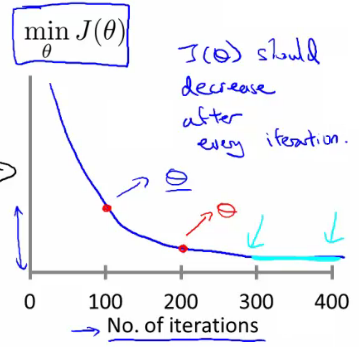
\includegraphics[width=0.6\textwidth]{resources/min_cost_function}

~\\
Automatic convergence tests

\begin{itemize}
\item Check if $J(\theta)$ changes by a small threshold or less.
\item Choosing this threshold is hard.
\item So often easier to check for a straight line.
\item Why? - Because we're seeing the straightness in the context of the whole algorithm.
\end{itemize}

~\\
If you plot $J(\theta)$ vs iterations and see the value is increasing - means you probably need a smaller $\alpha$.

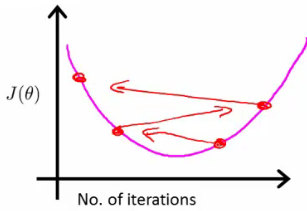
\includegraphics[width=0.5\textwidth]{resources/alpha_big}

~\\
However, you overshoot, therefore lower your learning rate so that you can reach the minimum (green line).\\

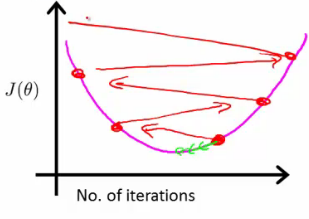
\includegraphics[width=0.5\textwidth]{resources/alpha_small}

\section*{Features and polynomial regression}

\begin{itemize}
\item May fit the data better.
\item Overfitting vs underfitting.
\end{itemize}

~\\
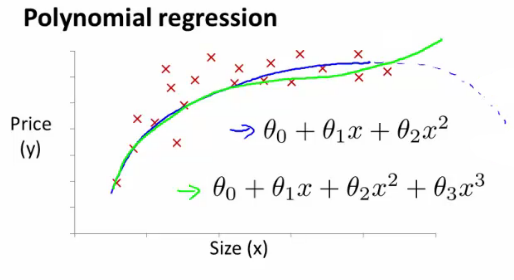
\includegraphics[width=0.8\textwidth]{resources/polynomial_regression}

\section*{Normal equation}

\begin{itemize}
\item The normal equation is a superior approach for some linear regression problems.
\item We've been using a gradient descent - iterative method that takes steps to convere.
\item Normal equation gives us $\theta$ analytically.
\end{itemize}

\subsection*{How does it work?}

\begin{itemize}
\item Here $\theta$ is an n+1 dimensional vector of real numbers.
\item Cost function is a function that takes that vector as an argument.
\item How do we minimize this function?
\item Take the partial derivative of $J(\theta)$ with respect $\theta_j$ and set to $0$ for every j. Solve for $\theta_0$ to $\theta_n$.
\end{itemize}

\subsection*{Example}

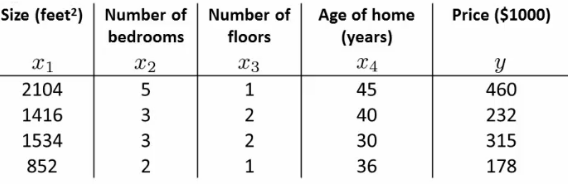
\includegraphics[width=\textwidth]{resources/normal_eq_table}

Steps
\begin{itemize}
\item $m=4$, $n=4$. 
\item Add an extra column ($x_0$ feature).
\item Construct a matrix (X - the design matrix) which contains all the training data features in an $[m \times n+1]$ matrix.
\item Construct a column vector y vector $[m x 1]$ matrix.
\item Use the following equation for $\theta$:
\end{itemize}

$$\theta = (X^TX)^{-1}X^Ty$$

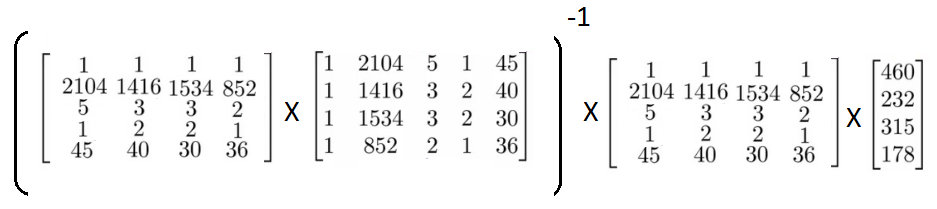
\includegraphics[width=\textwidth]{resources/normal_eq_matrix}

~\\
If you compute this, you get the value of theta which minimize the cost function.

\section*{Gradient descent vs normal equation}


\begin{table}[!htbp]
\bgroup
\def\arraystretch{1.5}%
\begin{tabular}{|c|c|}
 \hline
Gradient Descent & Normal Equation \\
 \hline
Need to chose learning rate &  No need to chose a learning rate \\
Needs many iterations - could make it slower & No need to iterate, check for convergence etc. \\
Works well even when n is massive (millions) & Slow of n is large \\
 \hline
\end{tabular}
\egroup
\end{table}

\end{document}